%============================================================
%  Capitolo 14 – Graph Neural Networks e Graph Convolutional Networks
%============================================================
\chapter{Graph Neural Networks}
\label{ch:gnn}

I \textbf{Graph Neural Networks} (GNN) sono una famiglia di modelli di
deep learning progettati per operare su dati strutturati come grafi.
A differenza di CNN e RNN, che assumono rispettivamente una griglia
regolare o una sequenza ordinata, le GNN sono in grado di gestire
strutture di connettività arbitrarie, sfruttando la topologia del
grafo per apprendere rappresentazioni ricche di nodi, archi e del
grafo nel suo insieme \citep{bishop2024}.

%------------------------------------------------------------
\section{Grafi come Strutture Dati}
\label{sec:graphs}

\subsection{Definizione e Attributi}
\label{subsec:graph-def}

Un \textbf{grafo} $G = (V, E)$ è una struttura dati composta da nodi
(vertici) e archi, privi di un inizio o una fine definiti. I grafi
possono essere \emph{diretti} (la direzione della connessione è
rilevante) o \emph{indiretti} (l'ordine non conta). I grafi diretti
possono essere unidirezionali o bidirezionali.

Ogni grafo è caratterizzato da tre tipi di attributi:

\begin{description}
  \item[$V$ — Vertex attributes] Attributi associati a ciascun nodo,
        ad esempio l'identità del nodo o il numero di vicini.
  \item[$E$ — Edge attributes] Attributi associati a ciascun arco,
        incluse la direzione, il peso o l'identità dell'arco.
  \item[$U$ — Global attributes] Attributi globali dell'intero grafo,
        detti anche \emph{master node} o \emph{context vector},
        ad esempio il numero totale di nodi o il cammino più lungo.
\end{description}

\begin{figure}[H]
  \centering
  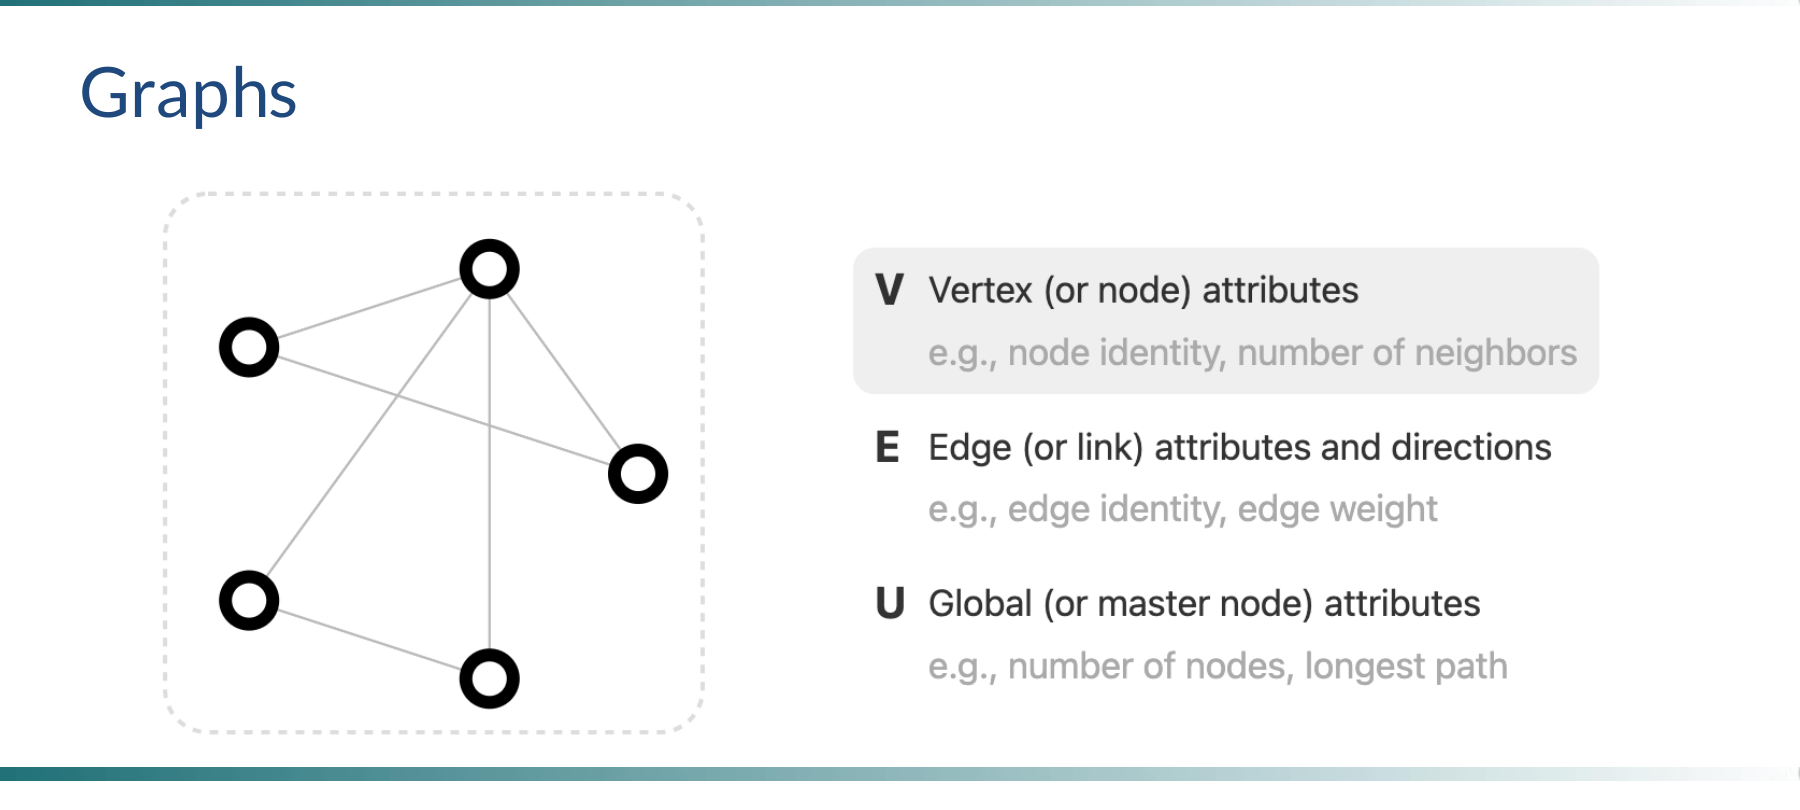
\includegraphics[width=0.82\linewidth]{figures/cf14_graph_attributes.png}
  \caption{Un grafo con i tre tipi di attributi: $V$ (nodi),
           $E$ (archi) e $U$ (globale). I nodi memorizzano
           proprietà locali, gli archi codificano relazioni,
           il vettore globale riassume proprietà dell'intero grafo.}
  \label{fig:graph_attributes}
\end{figure}

\subsection{Grafi in Natura: Esempi di Dominio}
\label{subsec:graph-examples}

I grafi modellano naturalmente numerosi tipi di dati reali:

\begin{description}
  \item[Immagini come grafi] Un'immagine può essere rappresentata come
        un grafo con struttura regolare, in cui ogni pixel è un nodo
        connesso via arco ai pixel adiacenti. Ogni nodo memorizza il
        vettore RGB del pixel. La matrice di adiacenza risultante ha
        una struttura a bande, poiché ogni pixel è connesso a un
        numero fisso di vicini (al massimo 8).
  \item[Testo come grafo] In una sequenza testuale ogni parola è un
        nodo connesso alla parola precedente e alla successiva. La
        matrice di adiacenza è puramente diagonale.
  \item[Molecole come grafi] Gli atomi sono nodi e i legami covalenti
        sono archi. La rappresentazione grafica è una comoda
        astrazione di un oggetto tridimensionale.
  \item[Reti sociali come grafi] Gli individui sono nodi e le loro
        relazioni sono archi. Permettono di studiare comportamenti
        collettivi di persone e organizzazioni.
\end{description}

\begin{figure}[H]
  \centering
  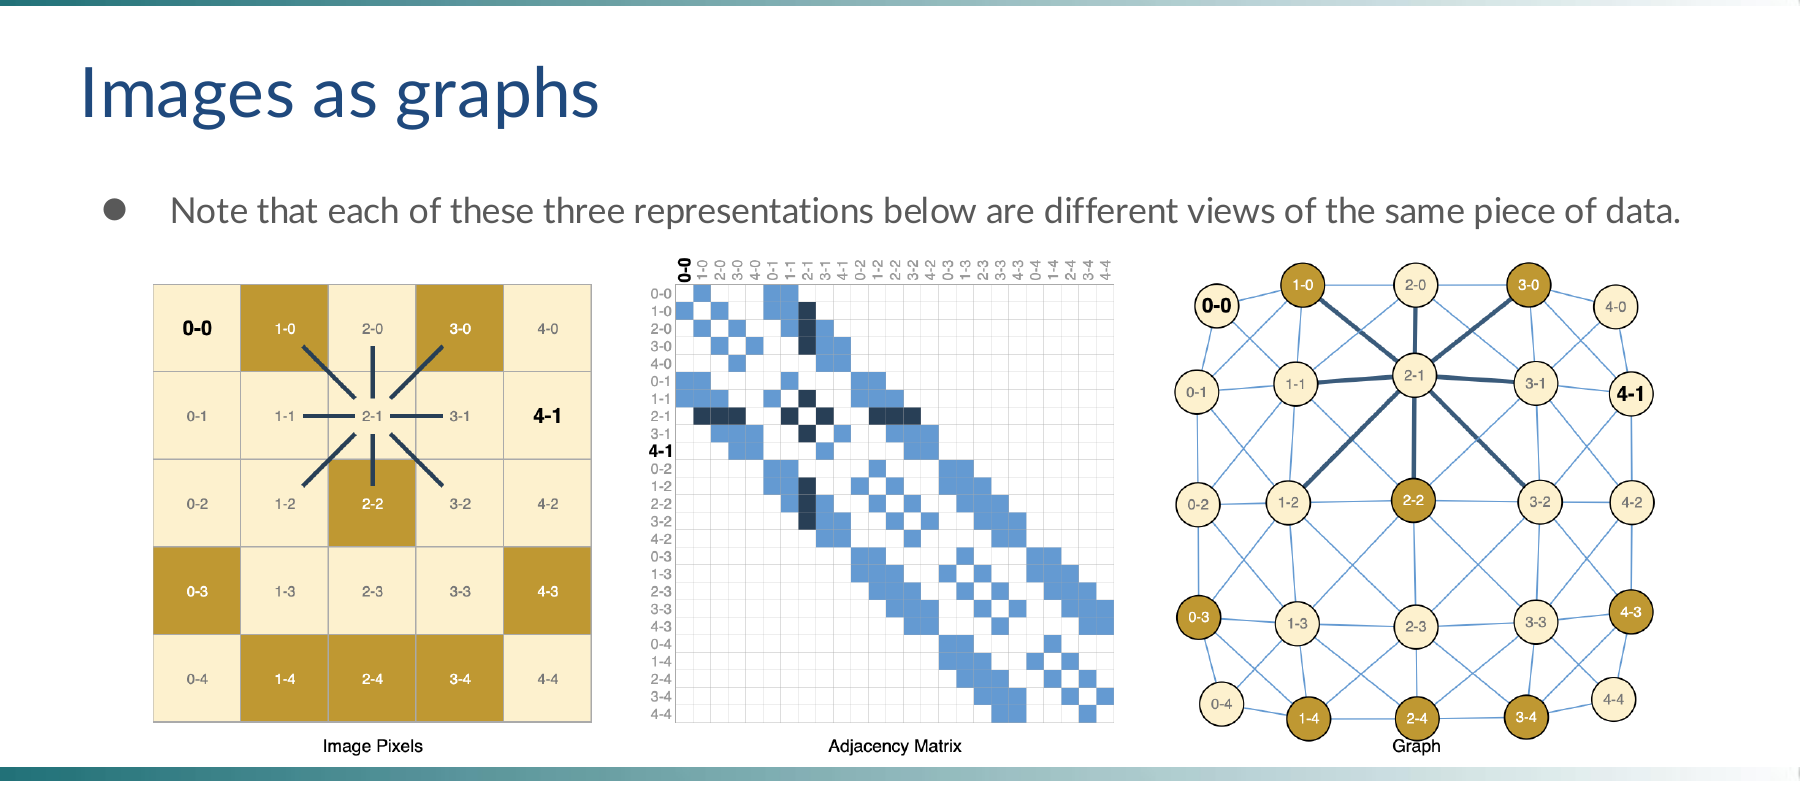
\includegraphics[width=0.92\linewidth]{figures/cf14_images_as_graphs.png}
  \caption{Tre rappresentazioni equivalenti della stessa immagine
           $5\times5$: l'immagine a pixel (sinistra), la matrice di
           adiacenza a bande (centro) e il grafo esplicito (destra).
           I nodi centrali dell'immagine hanno più connessioni rispetto
           ai nodi di bordo.}
  \label{fig:images_as_graphs}
\end{figure}

\subsection{Task su Grafi}
\label{subsec:graph-tasks}

I principali task di machine learning su grafi sono:

\begin{description}
  \item[Graph-level task] Predire una proprietà dell'intero grafo,
        ad esempio se una molecola è tossica o a cosa si lega.
        È l'analogo della classificazione di immagini con MNIST.
  \item[Node-level task] Predire l'identità o il ruolo di ciascun
        nodo. Un esempio classico è il \emph{Karate Club} di Zachary:
        classificare i membri in base all'allegiance a uno dei due
        club dopo una scissione politica. È analogo alla
        segmentazione semantica delle immagini.
  \item[Edge-level task] Predire le relazioni tra nodi (scene
        understanding) o l'esistenza di archi mancanti
        (link prediction).
  \item[Node Clustering] Raggruppare nodi simili sulla base della
        connettività.
  \item[Influence Maximization] Identificare i nodi più influenti
        in una rete.
\end{description}

\subsection{Dataset di Grafi Reali}
\label{subsec:graph-datasets}

\begin{figure}[H]
  \centering
  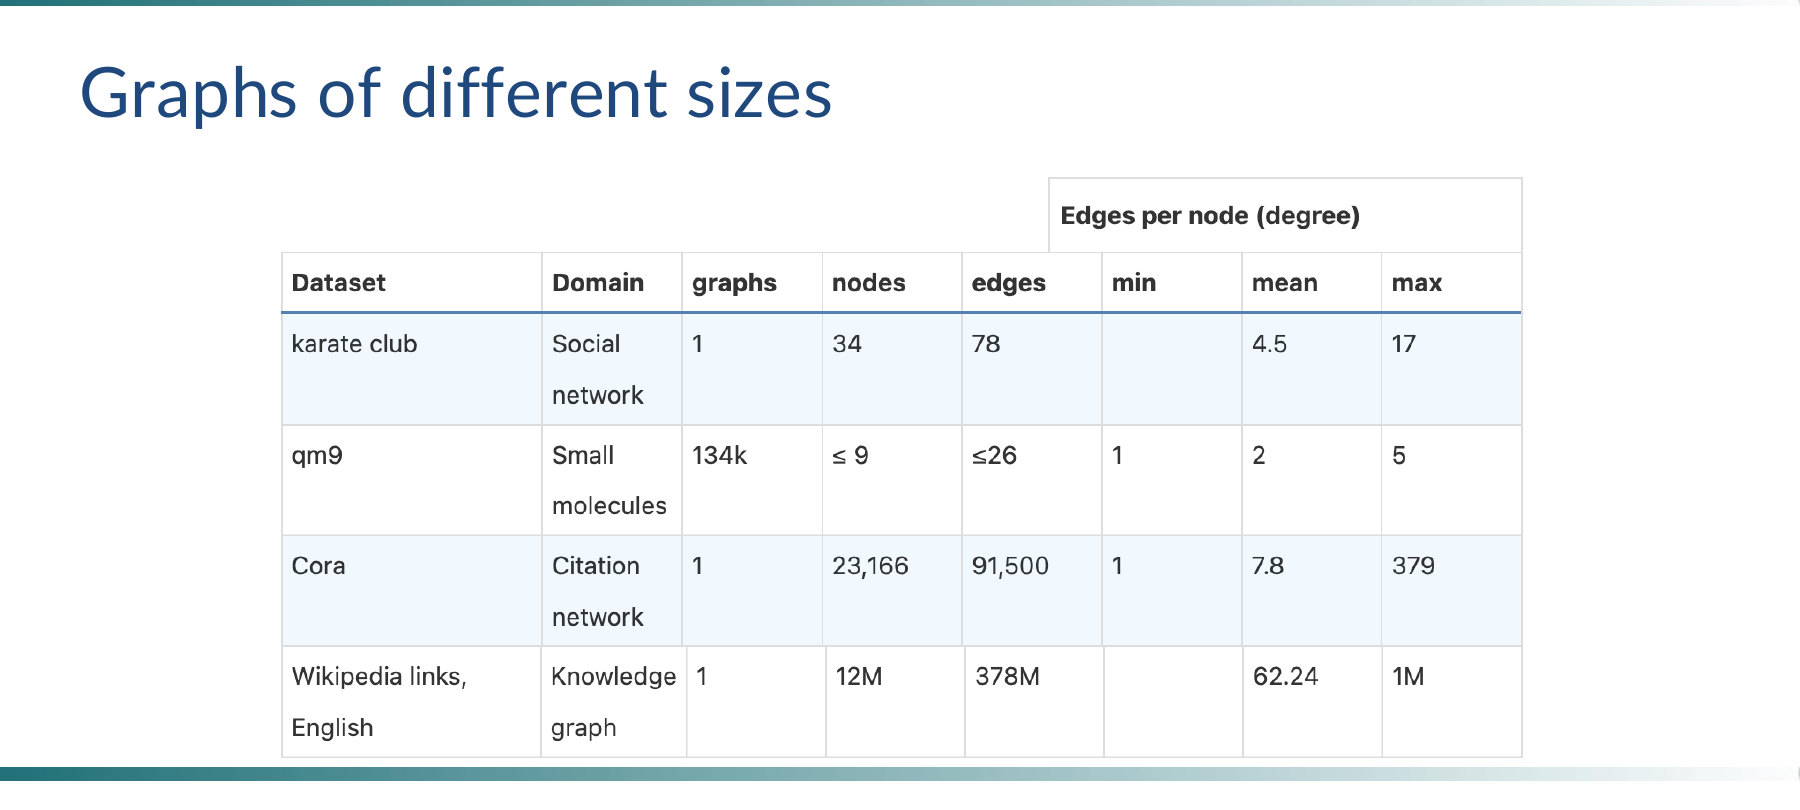
\includegraphics[width=0.82\linewidth]{figures/cf14_graph_datasets.png}
  \caption{Statistiche di dataset di grafi reali: il karate club
           (rete sociale, 34 nodi, 78 archi), QM9 (molecole piccole,
           $\leq9$ nodi, $\leq26$ archi), Cora (citation network,
           23\,166 nodi, 91\,500 archi), Wikipedia (knowledge graph,
           12M nodi, 378M archi).}
  \label{fig:graph_datasets}
\end{figure}

%------------------------------------------------------------
\section{Le Sfide del Calcolo su Grafi}
\label{sec:graph-challenges}

\subsection{Struttura Non Uniforme}
\label{subsec:irregular-structure}

I grafi sono modelli matematici estremamente flessibili, ma proprio
per questo mancano di una struttura uniforme tra istanze diverse.
Considerando la predizione di tossicità di molecole, emergono
immediatamente le seguenti difficoltà:

\begin{itemize}
  \item Le molecole possono avere numeri diversi di atomi.
  \item Gli atomi possono essere di tipo diverso.
  \item Ogni atomo può avere un numero diverso di connessioni.
  \item Le connessioni possono avere forze diverse.
\end{itemize}

\subsection{Node-Order Equivariance}
\label{subsec:equivariance}

Rappresentare un grafo come vettore richiede di fissare un ordinamento
dei nodi. Tuttavia, quando i nodi non hanno un ordine intrinseco, lo
stesso grafo può essere descritto da matrici di adiacenza diverse (una
per ogni permutazione dei nodi). Si desidera quindi che gli algoritmi
siano \textbf{node-order equivarianti}: non devono dipendere
dall'ordinamento scelto, e se i nodi vengono permutati, le
rappresentazioni risultanti devono essere permutate allo stesso modo.

\subsection{Scalabilità}
\label{subsec:scalability}

I grafi possono essere enormi (reti sociali con miliardi di utenti).
Fortunatamente, i grafi naturali sono \emph{sparsi}: il numero di archi
tende a crescere linearmente nel numero di nodi. Ciò permette di usare
metodi efficienti basati su \textbf{liste di adiacenza}, che evitano
di allocare l'intera matrice $n_{\text{nodes}}^2$.

\subsection{Rappresentazione con Liste di Adiacenza}
\label{subsec:adjacency-list}

\begin{figure}[H]
  \centering
  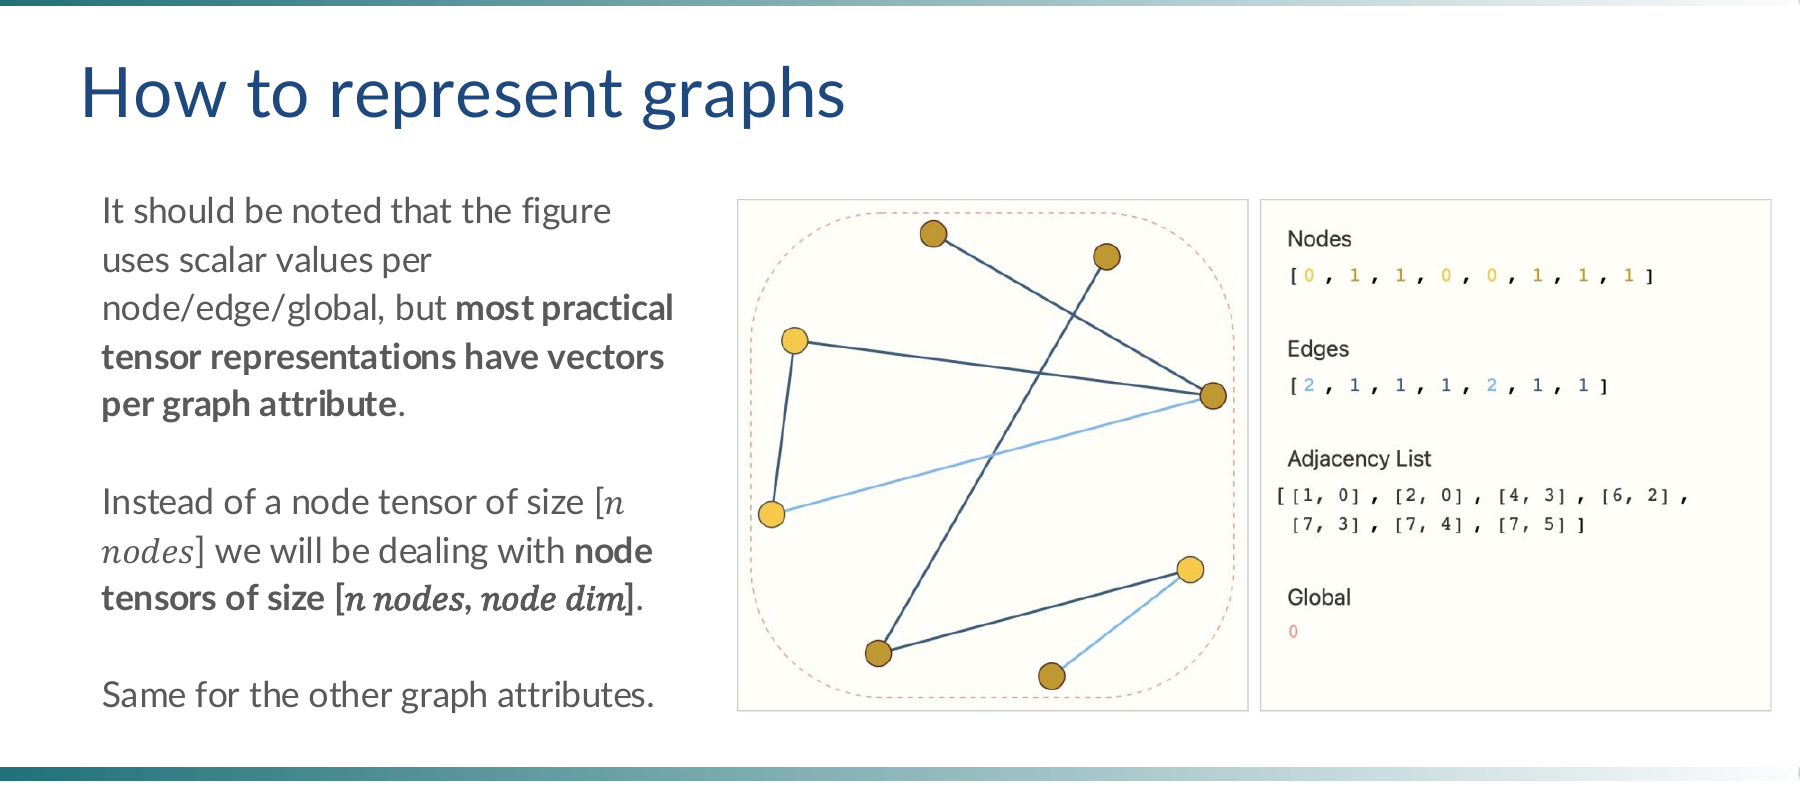
\includegraphics[width=0.88\linewidth]{figures/cf14_graph_representation.png}
  \caption{Rappresentazione di un grafo tramite lista di adiacenza.
           Ogni arco $e_k$ tra i nodi $n_i$ e $n_j$ è codificato
           come coppia $(i,j)$. In pratica ogni attributo di nodo è
           un tensore di dimensione $[n_{\text{nodes}},
           \text{node\_dim}]$ e ogni attributo di arco di dimensione
           $[n_{\text{edges}}, \text{edge\_dim}]$.}
  \label{fig:graph_representation}
\end{figure}

%------------------------------------------------------------
\section{Graph Neural Networks}
\label{sec:gnn-core}

\subsection{Definizione e Framework}
\label{subsec:gnn-def}

Una \textbf{GNN} è una trasformazione ottimizzabile su tutti gli
attributi del grafo (nodi, archi, contesto globale) che preserva le
simmetrie del grafo (invarianza alla permutazione dei nodi). Il
framework adottato è il \emph{message passing neural network}
(Gilmer et al., 2017) con la schematizzazione \emph{Graph Nets}
(Battaglia et al., 2018). Le GNN adottano un'architettura
\textbf{graph-in, graph-out}: accettano un grafo come input,
trasformano progressivamente gli embedding di nodi, archi e contesto
globale, senza modificare la connettività del grafo.

\subsection{La GNN più Semplice}
\label{subsec:simplest-gnn}

La GNN più semplice apprende nuovi embedding per tutti gli attributi
del grafo senza usare la connettività. Applica un MLP separato a
ogni componente:

\begin{itemize}
  \item Per ogni vettore nodo, l'MLP produce un nuovo vettore nodo.
  \item Per ogni arco, l'MLP produce un embedding per arco.
  \item Per il contesto globale, l'MLP produce un singolo embedding
        per l'intero grafo.
\end{itemize}

\begin{figure}[H]
  \centering
  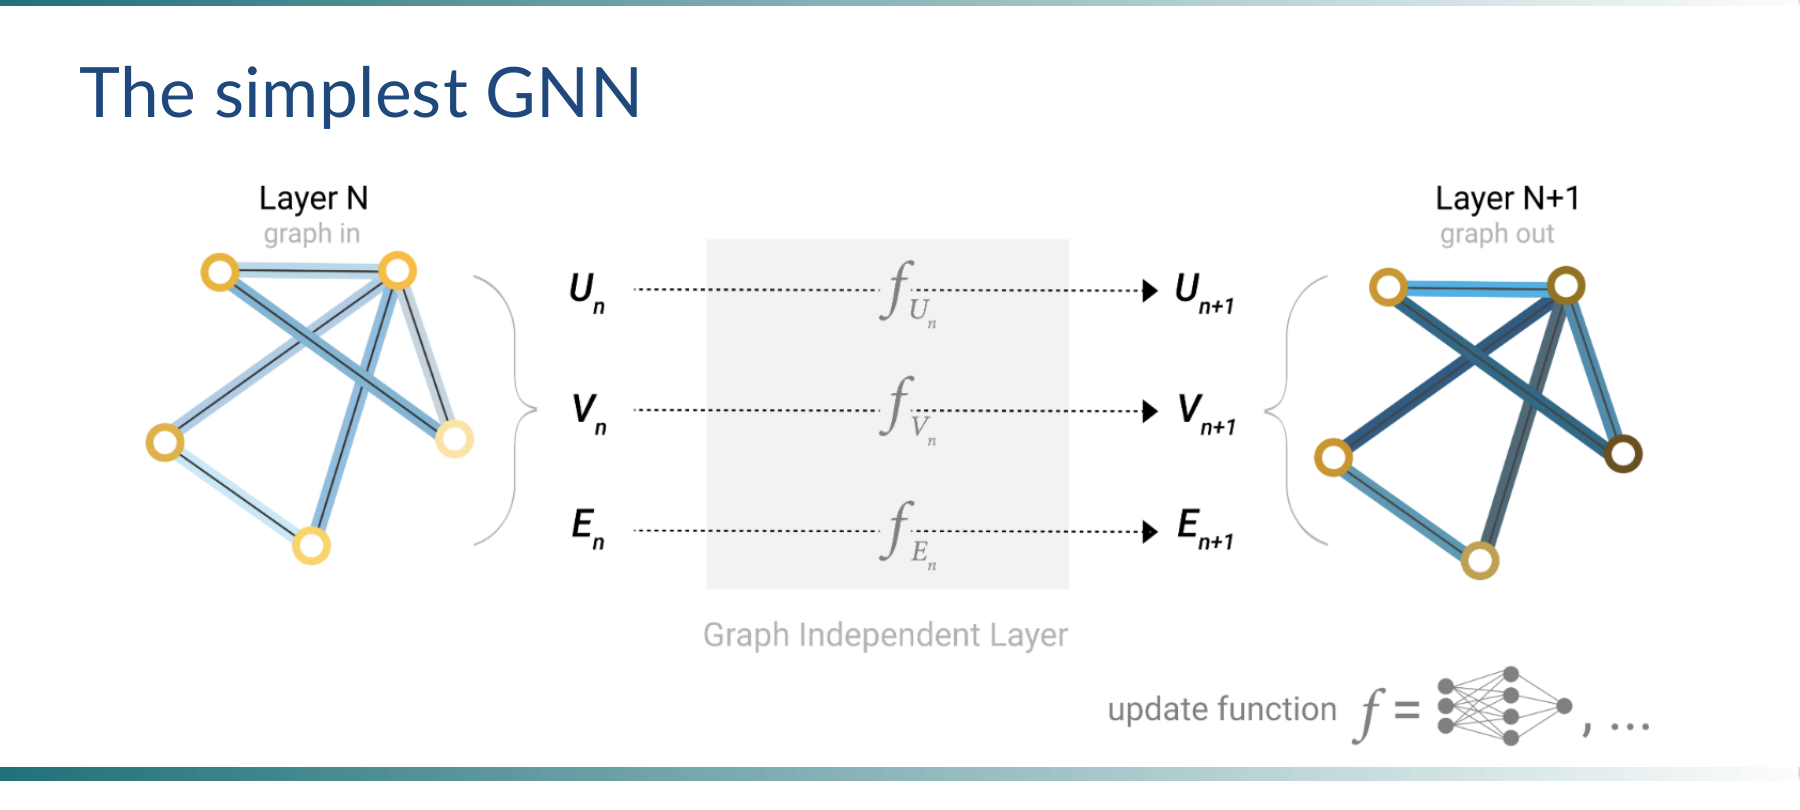
\includegraphics[width=0.88\linewidth]{figures/cf14_simplest_gnn.png}
  \caption{La GNN più semplice (Graph Independent Layer). Al layer $N$
           il grafo in ingresso ha attributi $U_n$, $V_n$, $E_n$;
           ciascuno è trasformato da una funzione di aggiornamento $f$
           (un MLP) indipendentemente dagli altri, producendo
           $U_{n+1}$, $V_{n+1}$, $E_{n+1}$ al layer $N+1$.}
  \label{fig:simplest_gnn}
\end{figure}

\subsection{Predizioni tramite Pooling}
\label{subsec:pooling}

Quando le informazioni necessarie per una predizione si trovano in un
attributo diverso da quello su cui si vuole predire, è necessario il
\textbf{pooling}. Il pooling si svolge in due passi:
\begin{enumerate}
  \item Per ogni elemento da aggregare, raccogliere tutti gli embedding
        e concatenarli in una matrice.
  \item Aggregare gli embedding raccolti, solitamente tramite somma.
\end{enumerate}

L'operazione di pooling è denotata con $\rho$, con il pedice che
indica la direzione del flusso (ad esempio $\rho_{E_n \to V_n}$
per aggregare archi verso nodi).

\subsection{Message Passing}
\label{subsec:message-passing}

Per rendere gli embedding consapevoli della connettività del grafo, si
introduce il \textbf{message passing}: i nodi (o archi) vicini si
scambiano informazioni e influenzano reciprocamente i propri embedding.
Il processo si articola in tre passi:

\begin{enumerate}
  \item Per ogni nodo, raccogliere tutti gli embedding dei nodi vicini
        (messaggi).
  \item Aggregare tutti i messaggi tramite una funzione (es.\ somma).
  \item Passare i messaggi aggregati attraverso una funzione di
        aggiornamento appresa (MLP).
\end{enumerate}

Applicando il message passing una volta si ottiene il più semplice
layer GNN con connettività. Impilando $K$ layer, un nodo incorpora
informazioni da tutti i nodi a distanza al più $K$ hop.

\begin{figure}[H]
  \centering
  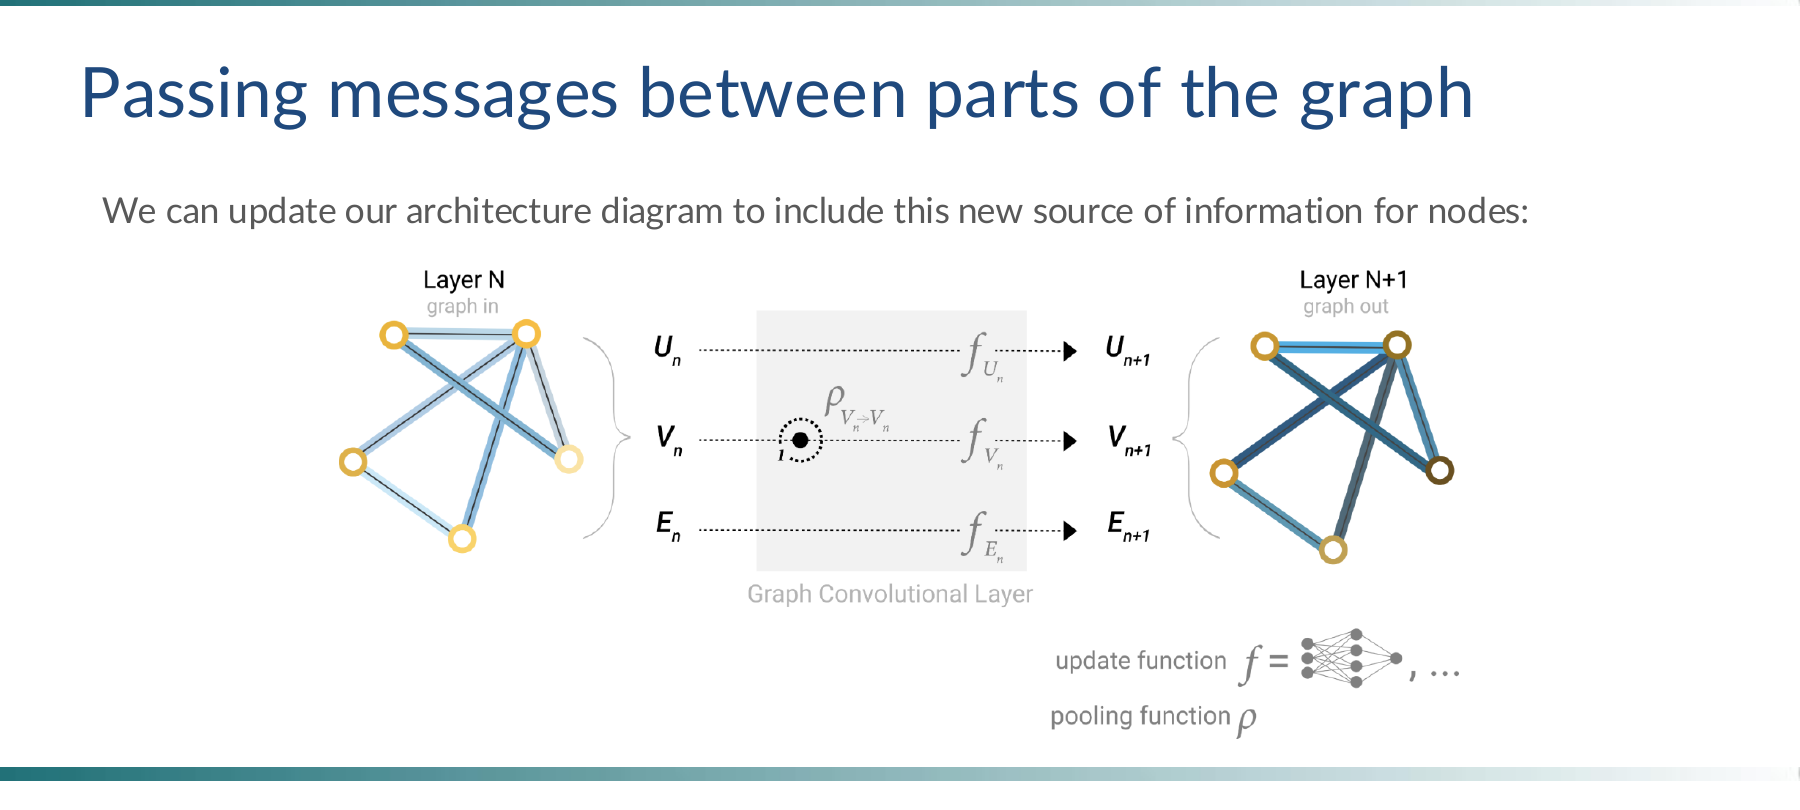
\includegraphics[width=0.92\linewidth]{figures/cf14_message_passing.png}
  \caption{Layer di Graph Convolutional con message passing. Il grafo
           al layer $N$ ha attributi $(U_n, V_n, E_n)$; la funzione
           di pooling $\rho_{V_n \to V_i}$ aggrega i vicini di ciascun
           nodo; la funzione di aggiornamento $f_{V_n}$ (MLP) produce
           i nuovi embedding $V_{n+1}$. Lo stesso avviene per $U$ e
           $E$.}
  \label{fig:message_passing}
\end{figure}

\subsection{Apprendimento di Rappresentazioni degli Archi}
\label{subsec:edge-repr}

Quando il dataset contiene solo informazioni sugli archi ma la
predizione deve essere fatta sui nodi, è possibile condividere
informazioni tra nodi e archi all'interno del layer GNN tramite
message passing. Le principali strategie di fusione sono:
concatenazione, mapping lineare dallo spazio degli archi a quello
dei nodi (o viceversa), o aggiornamento \emph{weave} che mantiene
quattro rappresentazioni aggiornate (nodo$\to$nodo, arco$\to$arco,
nodo$\to$arco, arco$\to$nodo).

\subsection{Rappresentazioni Globali}
\label{subsec:global-repr}

Un limite delle reti descritte finora è che nodi molto distanti
potrebbero non riuscire a scambiare informazioni in modo efficiente
anche con molti layer di message passing (con $K$ layer, l'informazione
si propaga al massimo $K$ hop). La soluzione adottata in Graph Nets
è il \textbf{vettore di contesto globale} $U$ (\emph{master node}),
connesso a tutti i nodi e archi della rete, che funge da canale di
comunicazione a lungo raggio.

\begin{figure}[H]
  \centering
  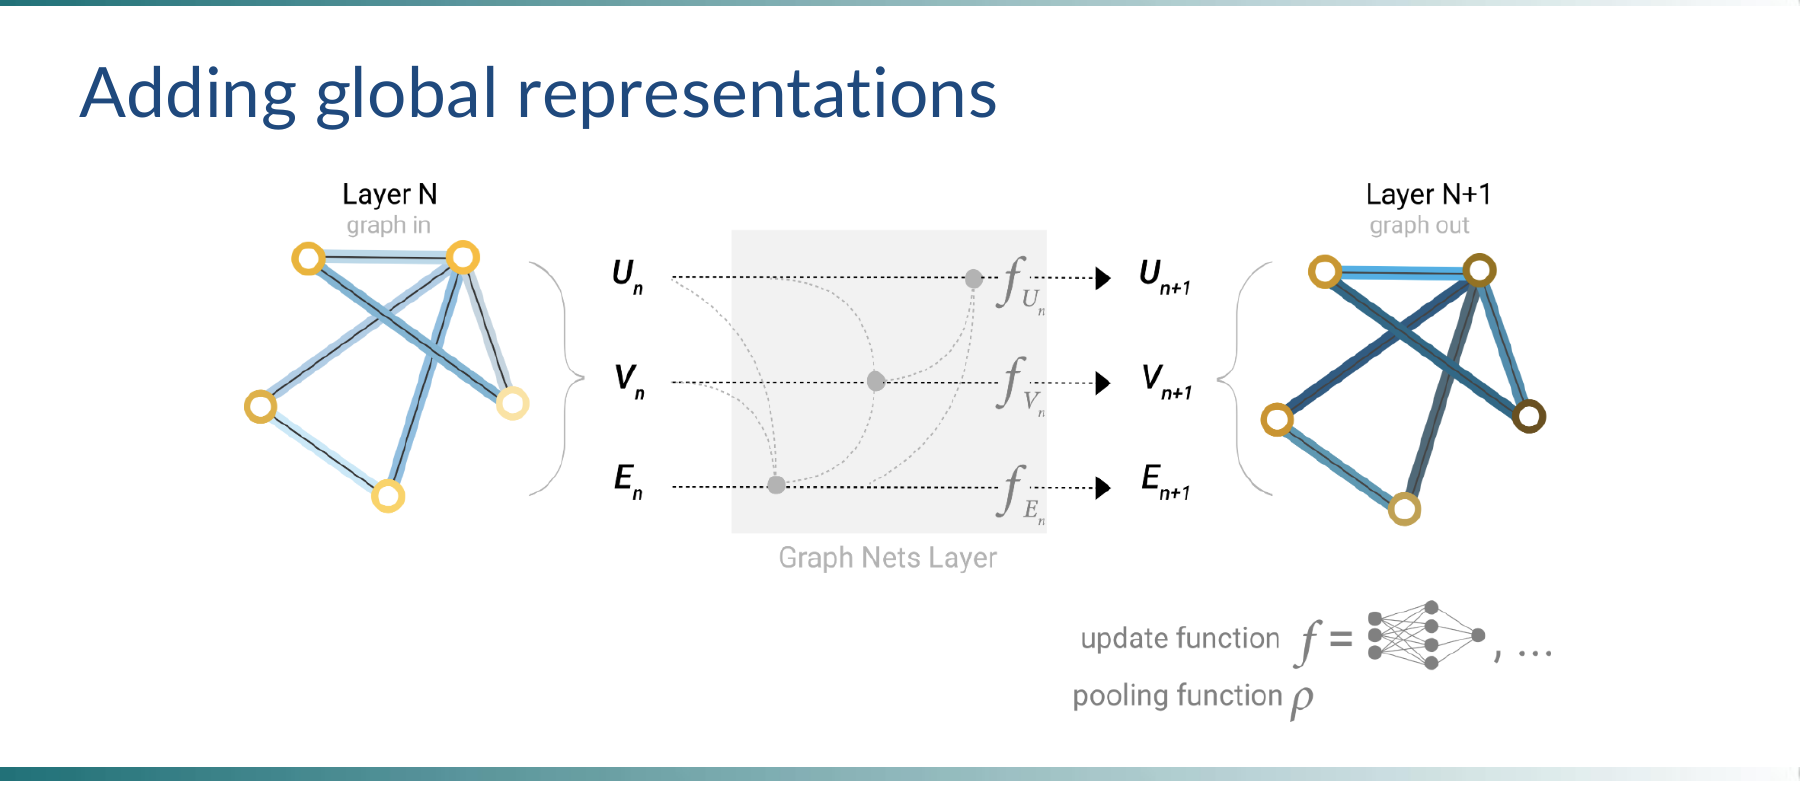
\includegraphics[width=0.92\linewidth]{figures/cf14_global_representations.png}
  \caption{Graph Nets Layer con rappresentazioni globali. Il vettore
           globale $U_n$ è connesso a tutti i nodi e archi, agendo da
           ponte per il trasferimento di informazioni a lungo raggio.
           Le funzioni di aggiornamento $f_{U_n}$, $f_{V_n}$,
           $f_{E_n}$ sono MLP condivisi.}
  \label{fig:global_repr}
\end{figure}

\subsection{Funzioni di Condizionamento}
\label{subsec:conditioning}

Con tutti gli attributi del grafo dotati di rappresentazioni apprese,
è possibile condizionare l'embedding di un nodo su tutte le sorgenti
di informazione disponibili: nodi vicini, archi connessi e
rappresentazione globale.

\begin{figure}[H]
  \centering
  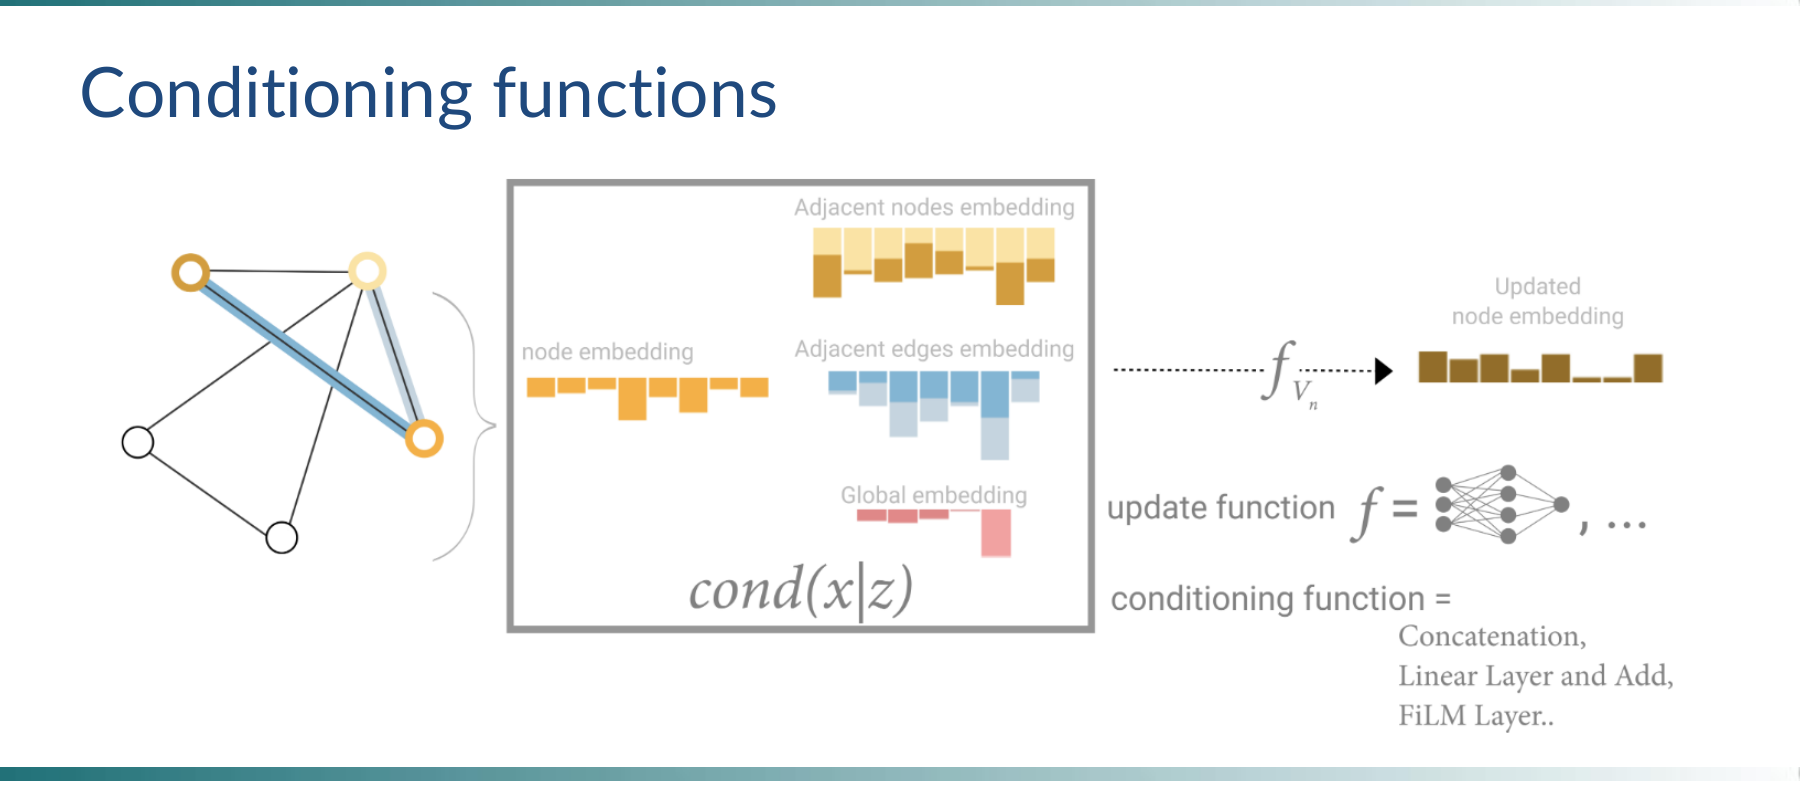
\includegraphics[width=0.88\linewidth]{figures/cf14_conditioning_functions.png}
  \caption{Funzione di condizionamento $\text{cond}(x|z)$ per un
           nodo. L'embedding del nodo viene concatenato con gli
           embedding degli archi adiacenti, dei nodi vicini e del
           vettore globale, quindi trasformato dall'update function
           $f_{V_n}$. Le opzioni di condizionamento includono
           concatenazione, layer lineare + add e FiLM layer.}
  \label{fig:conditioning}
\end{figure}

%------------------------------------------------------------
\section{GNN in a Nutshell: Formalizzazione}
\label{sec:gnn-math}

L'operazione matematica primaria in una GNN è lo schema di
\emph{message passing}, eseguito iterativamente su più layer.

\paragraph{Node Aggregation.} Per ogni nodo $i$, la funzione di
aggregazione combina le rappresentazioni dei nodi vicini $j$ e del
nodo corrente $i$:
\begin{equation}
  m_i^{(l)} = \sum_{j \in \mathcal{N}(i)}
  f^{(l)}\!\left(h_j^{(l-1)},\, h_i^{(l-1)},\, e_{ij}\right)
  \label{eq:gnn-aggregation}
\end{equation}
dove $h_i^{(l-1)}$ è la rappresentazione del nodo $i$ al layer
precedente, $e_{ij}$ è l'attributo dell'arco $(i,j)$ e $f^{(l)}$
è una funzione apprendibile.

\paragraph{Node Update.} I risultati dell'aggregazione vengono usati
per aggiornare la rappresentazione del nodo:
\begin{equation}
  h_i^{(l)} = g^{(l)}\!\left(h_i^{(l-1)},\, m_i^{(l)}\right)
  \label{eq:gnn-update}
\end{equation}
dove $g^{(l)}$ è una funzione apprendibile (tipicamente un MLP).

\paragraph{Graph-level Readout.} Una funzione di readout aggrega le
rappresentazioni dei nodi per ottenere una rappresentazione a livello
di grafo:
\begin{equation}
  h_G = \text{READOUT}\!\left(\left\{h_i^{(K)} \mid i \in V\right\}\right)
  \label{eq:gnn-readout}
\end{equation}

%------------------------------------------------------------
\section{Filtri Polinomiali e Graph Laplacian}
\label{sec:spectral}

\subsection{Il Graph Laplacian}
\label{subsec:laplacian}

Dato un grafo $G$ con $n$ nodi, sia $A$ la matrice di adiacenza
$0$-$1$ e $D$ la matrice diagonale dei gradi, dove
$D_{vv} = \sum_u A_{vu}$. Il \textbf{Graph Laplacian} è definito come:
\begin{equation}
  L = D - A
  \label{eq:laplacian}
\end{equation}

$L$ è il discreto analogo dell'operatore Laplaciano. È
\emph{positivo semidefinito} (tutti gli autovalori $\geq 0$) e
codifica la stessa informazione della matrice di adiacenza $A$:
dati $A$ o $L$, è possibile ricostruire l'altro. Il Laplacian
compare in numerosi problemi matematici su grafi: random walks,
spectral clustering, diffusione.

\begin{figure}[H]
  \centering
  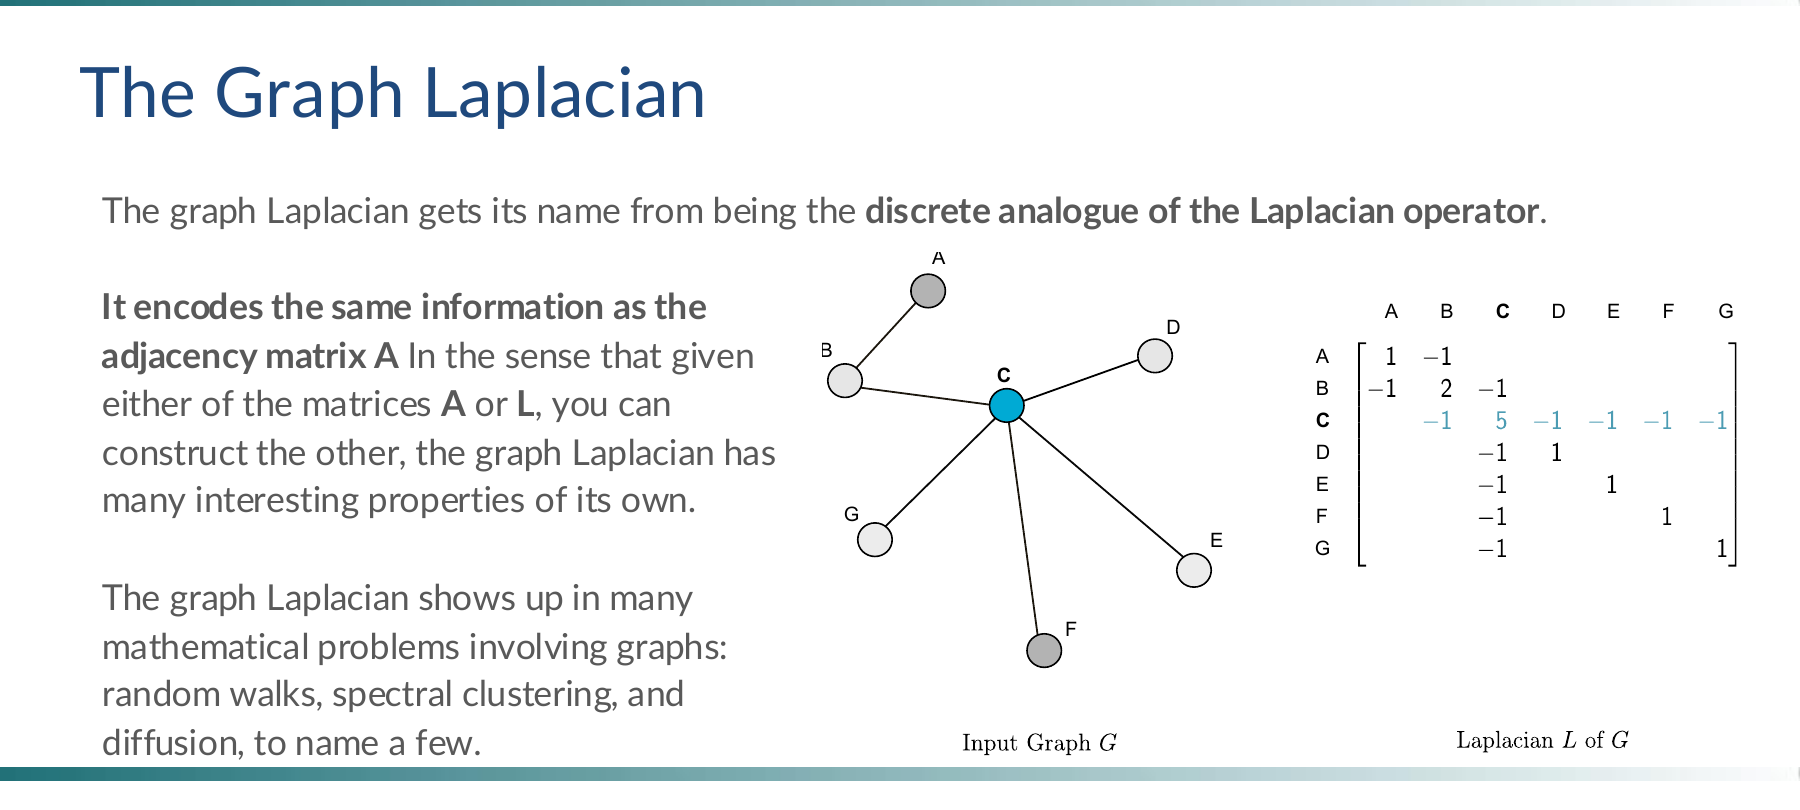
\includegraphics[width=0.88\linewidth]{figures/cf14_graph_laplacian.png}
  \caption{Un grafo $G$ con 7 nodi (sinistra) e la sua matrice
           Laplaciana $L = D - A$ (destra). Il nodo $C$, avente
           grado 5, ha $L_{CC} = 5$; gli archi incidenti in $C$
           producono $-1$ nelle posizioni corrispondenti. La riga
           highlighted (turchese) mostra la riga di $C$ nella
           matrice $L$.}
  \label{fig:graph_laplacian}
\end{figure}

\subsection{Filtri Polinomiali}
\label{subsec:poly-filters}

Si possono costruire \textbf{filtri polinomiali} del Laplacian della
forma:
\begin{equation}
  p_w(L) = \sum_{d=0}^{D} w_d\, L^d
  \label{eq:poly-filter}
\end{equation}

I coefficienti $w = [w_0, \ldots, w_D]$ sono i pesi appresi del
filtro, analogi ai pesi dei filtri nelle CNN. La convoluzione del
segnale $x \in \mathbb{R}^n$ (vettore delle feature dei nodi) con
il filtro $p_w$ è:
\begin{equation}
  x' = p_w(L)\, x
  \label{eq:poly-conv}
\end{equation}

La potenza $L^d$ ha la proprietà che $(L^d)_{vu} \neq 0$ solo se il
nodo $u$ è a distanza al più $d$ hop dal nodo $v$. Pertanto, il
filtro polinomiale di grado $d$ è \textbf{localizzato}: la
convoluzione al nodo $v$ coinvolge solo i nodi a distanza al massimo
$d$ hop. Il grado controlla la localizzazione.

\subsection{ChebNet}
\label{subsec:chebnet}

\textbf{ChebNet} (Defferrard et al., 2016) raffina i filtri
polinomiali usando i polinomi di Chebyshev di primo tipo $T_i$
applicati al Laplacian normalizzato $\tilde{L}$:
\begin{equation}
  p_w(\tilde{L}) = \sum_{i=0}^{D} w_i\, T_i(\tilde{L}),
  \qquad
  \tilde{L} = \frac{2L}{\lambda_{\max}(L)} - I
  \label{eq:chebnet}
\end{equation}

La normalizzazione garantisce che gli autovalori di $\tilde{L}$ siano
nell'intervallo $[-1, 1]$, prevenendo l'esplosione delle potenze di
$L$. I polinomi di Chebyshev assicurano stabilità numerica
nell'interpolazione. I filtri polinomiali sono node-order equivarianti
per costruzione (la somma sulle feature dei vicini non dipende
dall'ordine).

\paragraph{Embedding computation.} Impilando $K$ layer di ChebNet
con non-linearità, si ottiene una rete profonda in cui il $k$-esimo
layer ha i propri pesi appresi $w^{(k)}$:
\begin{equation}
  x^{(k)} = \sigma\!\left(p_{w^{(k)}}(\tilde{L})\, x^{(k-1)}\right)
  \label{eq:chebnet-stacked}
\end{equation}

I pesi del filtro sono condivisi tra tutti i nodi, esattamente come
il weight-sharing nelle CNN su griglia.

%------------------------------------------------------------
\section{Architetture GNN Moderne}
\label{sec:modern-gnn}

\subsection{Graph Convolutional Networks (GCN)}
\label{subsec:gcn}

Le \textbf{Graph Convolutional Networks} (Kipf \& Welling, 2017)
semplificano ChebNet limitando il filtro al primo ordine ($D=1$) e
applicando un'ulteriore normalizzazione simmetrica. La regola di
propagazione al layer $k$ è:

\begin{equation}
  h_v^{(k)} = f^{(k)}\!\left(
    W^{(k)} \cdot \frac{\sum_{u \in \mathcal{N}(v)} h_u^{(k-1)}}{|\mathcal{N}(v)|}
    + B^{(k)} \cdot h_v^{(k-1)}
  \right)
  \quad \forall\, v \in V
  \label{eq:gcn}
\end{equation}

dove $h_v^{(k)}$ è l'embedding del nodo $v$ al layer $k$,
$\mathcal{N}(v)$ è il vicinato di $v$, $W^{(k)}$ e $B^{(k)}$ sono
matrici di peso apprendibili e $f^{(k)}$ è una funzione non lineare.

\begin{figure}[H]
  \centering
  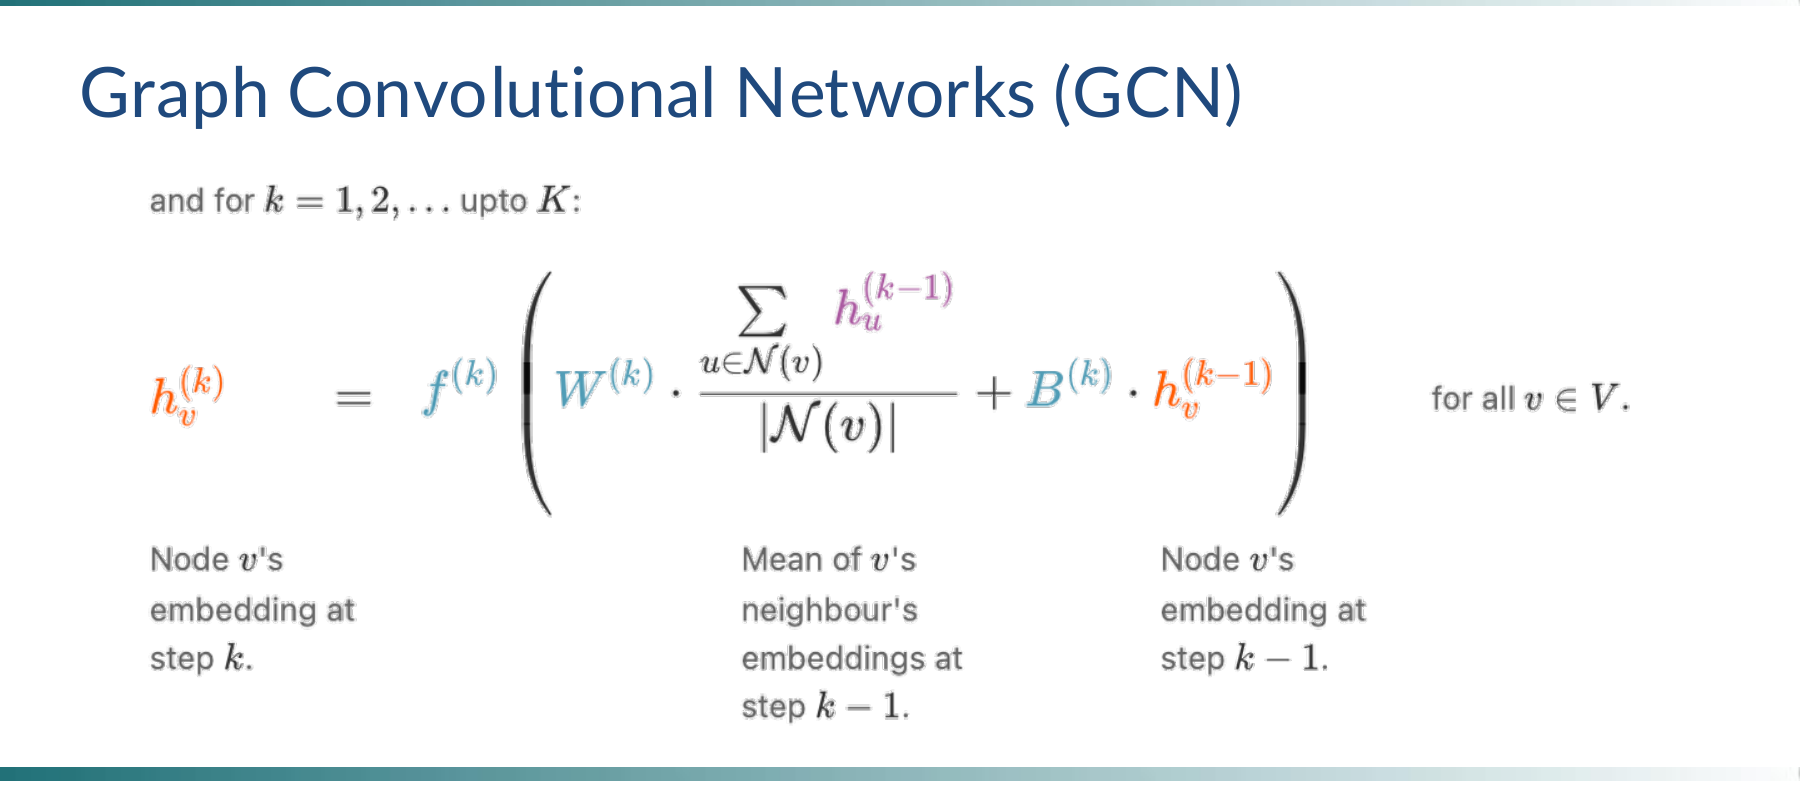
\includegraphics[width=0.88\linewidth]{figures/cf14_gcn_equation.png}
  \caption{Equazione di propagazione GCN. L'embedding
           $h_v^{(k)}$ (rosso) è una funzione apprendibile
           $f^{(k)}$ della media pesata degli embedding dei vicini
           (viola) e dell'embedding del nodo stesso al layer
           precedente (arancione). I pesi $W^{(k)}$ e $B^{(k)}$
           sono condivisi tra tutti i nodi, garantendo la scalabilità
           del modello.}
  \label{fig:gcn_equation}
\end{figure}

La normalizzazione GCN originale usa $\hat{A} = \tilde{D}^{-1/2}
\tilde{A}\, \tilde{D}^{-1/2}$ con $\tilde{A} = A + I$ (aggiunta di
auto-loop), più stabile dell'aggregazione semplice al denominatore.
La predizione finale è:
\begin{equation}
  \hat{y}_v = \text{PREDICT}\!\left(h_v^{(K)}\right)
  \label{eq:gcn-predict}
\end{equation}

\paragraph{Vantaggi GCN.} Il numero di parametri del modello
(proporzionale a $\text{node\_dim}^2 \times K$) è indipendente dalla
dimensione del grafo, garantendo buona scalabilità.

\paragraph{GCN in a nutshell.}
\begin{enumerate}
  \item \textbf{Node Aggregation}: somma pesata delle feature dei
        nodi vicini con normalizzazione per il grado:
        $\sum_{j \in \mathcal{N}(i)} \frac{h_j^{(l-1)}}{\sqrt{d_i\, d_j}}$
  \item \textbf{Node Update}: applicazione di trasformazione lineare
        e attivazione non lineare:
        $h_i^{(l)} = \sigma\!\left(W^{(l)} \cdot \text{AGG}_i\right)$
\end{enumerate}

\subsection{Graph Attention Networks (GAT)}
\label{subsec:gat}

Le \textbf{Graph Attention Networks} (Veličković et al., 2018)
sostituiscono l'aggregazione con pesi uniformi con un meccanismo
di \textbf{attenzione} appreso:

\begin{equation}
  h_v^{(k)} = f^{(k)}\!\left(
    W^{(k)} \cdot \left[
      \sum_{u \in \mathcal{N}(v)} \alpha_{vu}^{(k-1)}\, h_u^{(k-1)}
      + \alpha_{vv}^{(k-1)}\, h_v^{(k-1)}
    \right]
  \right)
  \quad \forall\, v \in V
  \label{eq:gat}
\end{equation}

\begin{figure}[H]
  \centering
  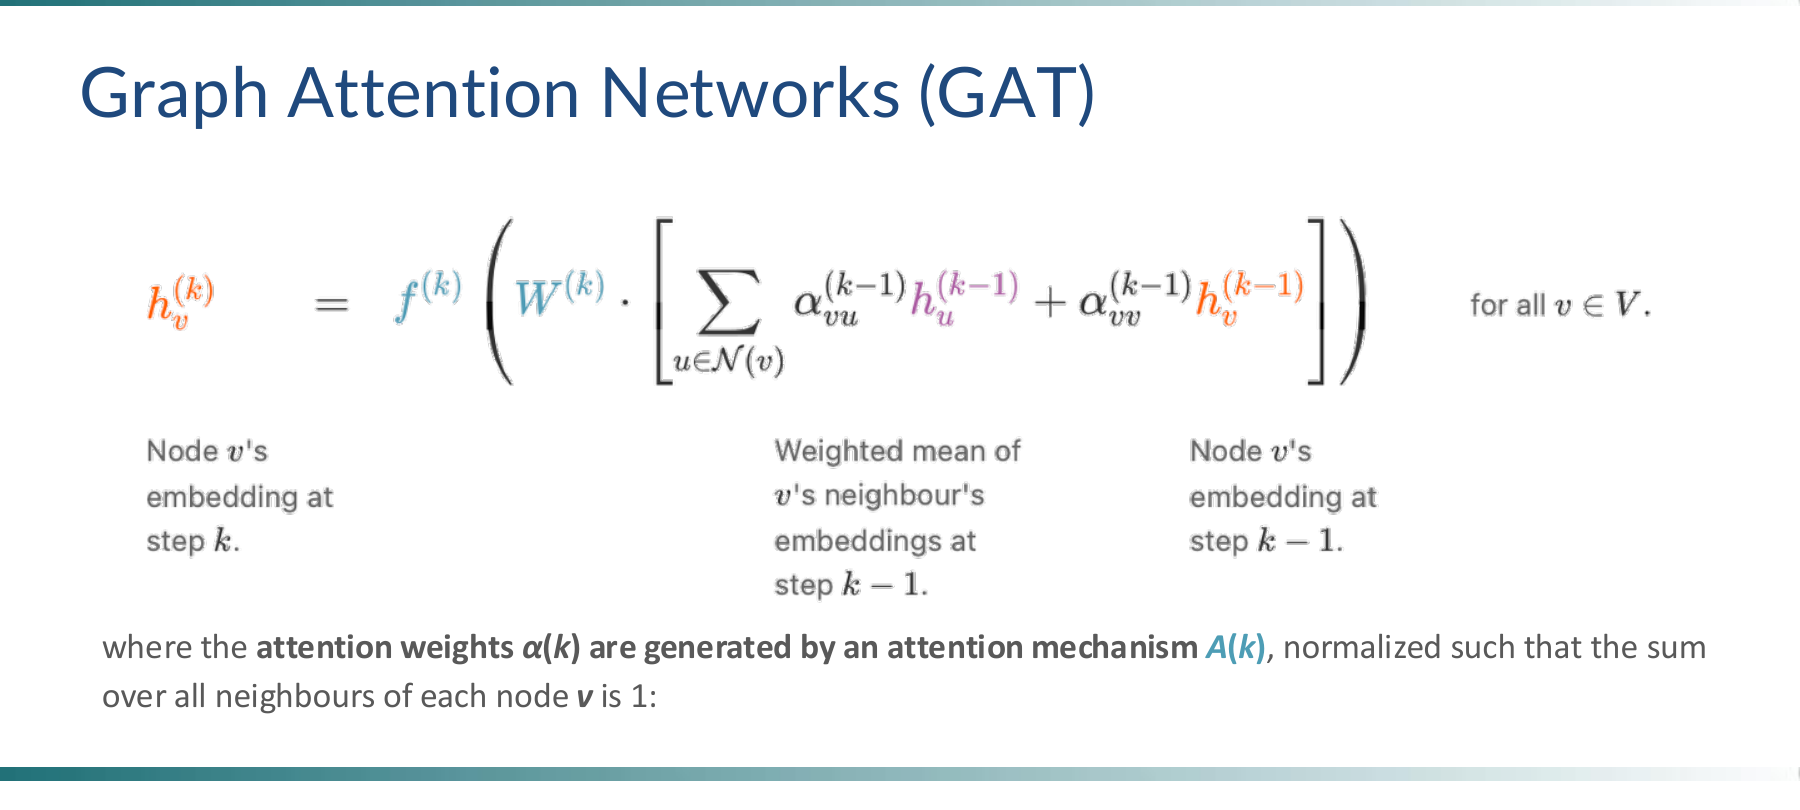
\includegraphics[width=0.88\linewidth]{figures/cf14_gat_equation.png}
  \caption{Equazione di propagazione GAT. I pesi di attenzione
           $\alpha_{vu}^{(k-1)}$ (generati dal meccanismo $A^{(k)}$,
           tipicamente un MLP) ponderano il contributo di ciascun
           vicino all'embedding del nodo. La sommatoria normalizzata
           su tutti i vicini produce la media pesata per attenzione.}
  \label{fig:gat_equation}
\end{figure}

I pesi $\alpha_{vu}^{(k)}$ sono generati da un meccanismo di
attenzione $A^{(k)}$ (spesso un piccolo MLP) e normalizzati con
softmax affinché la loro somma su tutti i vicini di $v$ sia 1:
\begin{equation}
  \sum_{u \in \mathcal{N}(v)} \alpha_{vu}^{(k)} + \alpha_{vv}^{(k)} = 1
  \label{eq:gat-norm}
\end{equation}

La variante discussa utilizza attenzione single-head; la variante
multi-head è analoga.

\subsection{GraphSAGE}
\label{subsec:graphsage}

\textbf{GraphSAGE} (Hamilton et al., 2017) introduce due innovazioni
rispetto a GCN: la scelta esplicita della funzione di aggregazione
e il \emph{neighbourhood sampling}.

La regola di aggiornamento è:
\begin{equation}
  h_v^{(k)} = f^{(k)}\!\left(
    W^{(k)} \cdot \left[h_v^{(k-1)},\, \text{AGG}\!\left(\left\{h_u^{(k-1)}\right\}_{u \in \mathcal{N}(v)}\right)\right]
  \right)
  \label{eq:graphsage}
\end{equation}

Le principali scelte per $\text{AGG}$ sono:
\begin{description}
  \item[Mean] Media degli embedding dei vicini (simile a GCN).
  \item[Max] Massimo elemento per elemento
        (\emph{dimension-wise maximum}).
  \item[LSTM] Aggregazione tramite LSTM dopo un ordinamento casuale
        dei vicini; più espressiva ma non equivariante senza
        ordinamento deterministico.
\end{description}

Il \textbf{neighbourhood sampling} campiona un sottoinsieme di
dimensione fissa del vicinato ad ogni step, indipendentemente
dalla dimensione reale del vicinato. Ciò aumenta la varianza degli
embedding ma rende GraphSAGE applicabile a grafi molto grandi.

\subsection{Graph Isomorphism Network (GIN)}
\label{subsec:gin}

Le \textbf{Graph Isomorphism Networks} (Xu et al., 2019) sono
state progettate per essere massimamente espressive, raggiungendo
il limite superiore teorico del test di isomorfismo
di Weisfeiler-Leman (WL). La regola di aggiornamento è:

\begin{equation}
  h_v^{(k)} = f^{(k)}\!\left(
    \left(1 + \epsilon^{(k)}\right) h_v^{(k-1)}
    + \sum_{u \in \mathcal{N}(v)} h_u^{(k-1)}
  \right)
  \label{eq:gin}
\end{equation}

dove $\epsilon^{(k)}$ è un parametro reale apprendibile (o fissato
a 0). L'idea chiave è che la funzione di aggregazione deve essere
\emph{iniettiva} per distinguere strutture locali diverse; la somma
(a differenza della media o del massimo) preserva questa proprietà
in spazi di feature discreti.

%------------------------------------------------------------
\section{Confronto tra Architetture GNN}
\label{sec:gnn-comparison}

\begin{table}[H]
  \centering
  \caption{Confronto tra le principali architetture GNN moderne.}
  \label{tab:gnn-comparison}
  \small
  \begin{tabularx}{\linewidth}{l X c l X}
    \toprule
    \textbf{Modello} & \textbf{Aggregazione}
      & \textbf{Att.} & \textbf{Espressività} & \textbf{Note} \\
    \midrule
    GCN       & Media normalizzata       & No           & Media       & Semplice, efficiente \\
    GAT       & Media pesata (attention) & Sì (appresa) & Alta        & Multi-head disponibile \\
    GraphSAGE & Mean / Max / LSTM        & No           & Media--Alta & Neighbourhood sampling \\
    GIN       & Somma + $\epsilon$       & No           & Massima (WL)& Teoricamente ottimale \\
    ChebNet   & Filtro polinomiale       & No           & Alta        & Base spettrale \\
    \bottomrule
  \end{tabularx}
\end{table}

\paragraph{Considerazioni pratiche.}
\begin{enumerate}
  \item \textbf{GCN} è il punto di partenza standard: semplice,
        stabile e scalabile. Preferirlo come baseline.
  \item \textbf{GAT} è preferibile quando si sospetta che i vicini
        abbiano importanza diversa; il costo computazionale è
        moderatamente superiore a GCN.
  \item \textbf{GraphSAGE} è la scelta naturale per grafi molto
        grandi (milioni di nodi) grazie al neighbourhood sampling
        e all'inductive learning.
  \item \textbf{GIN} è preferibile quando l'espressività è critica
        (es.\ task di graph isomorphism); richiede più attenzione
        alla regolarizzazione.
  \item Il numero di layer $K$ controlla il \emph{receptive field}:
        con $K$ layer ogni nodo incorpora informazioni da distanza
        al più $K$ hop. Valori tipici sono $K = 2$--$4$; aumentare
        $K$ può causare \emph{over-smoothing}.
  \item Per task \textbf{graph-level}, aggiungere una funzione di
        readout globale (sum/mean pooling o differentiable pooling).
  \item Per task \textbf{node-level} e \textbf{edge-level}, applicare
        direttamente un classificatore lineare agli embedding finali.
\end{enumerate}
